\documentclass[preprint,11pt,3p]{elsarticle} %review, or preprint

\usepackage{amssymb}
\usepackage{graphics}
\usepackage{float}
\usepackage[normalem]{ulem}
\usepackage{color}
\usepackage{lscape}

%Flowcharts
\usepackage[latin1]{inputenc}
\usepackage{tikz}
\usetikzlibrary{shapes,arrows}
% Define block styles
\tikzstyle{decision} = [diamond, draw, fill=blue!20, 
    text width=4.5em, text badly centered, node distance=3cm, inner sep=0pt]
\tikzstyle{block} = [rectangle, draw, fill=blue!20, 
    text width=5em, text centered, rounded corners, minimum height=4em]
\tikzstyle{line} = [draw, -latex']
\tikzstyle{cloud} = [draw, ellipse,fill=red!20, node distance=3cm,
    minimum height=2em]


%Some code to display the units after the equation 
\usepackage{mathtools}
\makeatletter
\providecommand\add@text{}
\newcommand\tagaddtext[1]{%
  \gdef\add@text{#1\gdef\add@text{}}}% 
\renewcommand\tagform@[1]{%
  \maketag@@@{\llap{\add@text\quad}(\ignorespaces#1\unskip\@@italiccorr)}%
}
\makeatother



\graphicspath{{./Images/}}

\journal{PVSEC Conference}

\begin{document}

\begin{frontmatter}

\title{Energy performance of PV modules as adaptive building shading systems} 

\author[ita]{P. Jayathissa\corref{cor2}}
    \ead{jayathissa@arch.ethz.ch}
\address[ita]{Architecture and Building Systems, Institute of Technology in Architecture, Department of Architecture, ETH Zurich, Switzerland} 
% For whatever reason the affiliation needs to be defined after the authors. Otherwise the numbering gets messed up.

\author[ita]{J. Schmidli}
    \ead{schmidje@student.ethz.ch}

\author[ita]{J. Hofer}
    \ead{hofer@arch.ethz.ch}


\author[ita]{A. Schlueter \corref{cor1} }
    \ead{schlueter@arch.ethz.ch}


\cortext[cor2]{Corresponding author}


\begin{abstract}
Shading systems improve building energy performance by controlling solar gains and natural lighting. Integrating photovoltaics opens new opportunities for building integrated photovoltaics by combining the benefits of adaptive shading with facade integrated solar tracking. Furthermore, it reduces the building energy demand and simultaneously generates electricity on-site. This paper presents a methodology for simulating the photovoltaic electricity production of a dynamic facade mounted PV system in combination with the energy consumption of a building through shading.
The simulation is conducted within the parametric Rhino / Grasshopper environment using Ladybug radiation analysis for the calculation of PV electricity generation. Building energy analysis is conducted through DIVA / EnergyPlus. From this simulation we can determine the optimum hourly position and orientation of the PV panels, not only for optimal energy harvest, but also for the overall balance of the room.

\end{abstract}

\begin{keyword}
Dynamic Photovoltaics \sep Multi Functional Envelope \sep BIPV \sep Adaptive Shading
\end{keyword}

\end{frontmatter}

\section{Introduction}
\label{ch:introduction}
% !TEX root = 99_main.tex

Buildings are at the heart of society and currently account for 32\% of global final energy consumption and 19\% of energy related greenhouse gas emissions \cite{IPCC}. Nevertheless the building sector has a 50-90\% emission reduction potential using existing technologies \cite{IPCC}. Within this strategy, building integrated photovoltaics (BIPV) has the potential of providing a substantial segment of a building's energy needs \cite{defaix2012technical}. Even the photovoltaic (PV) industry has identified BIPV as one of the four key factors for the future success of PV \cite{raugei2009life}. \\

%Recent developments regarding efficiency and costs of thin film BIPV technologies, in particular, CIGS, have brought new design possibilities \cite{NREL} \cite{kushiya2014cis} \cite{kaelin2004low} \cite{jelle2012building}. Their lightweight nature and customisable shapes allow for easier and more aesthetically pleasing integration into the building envelope. In addition, less power is required to actuate them, thus facilitating the development of dynamic envelope elements \cite{rossi2012adaptive}. \\


Dynamic building envelopes have gained interest in recent years because they can save energy by controlling direct and indirect radiation into the building, while still responding to the desires of the user \cite{loonen2013climate}. This mediation of solar insolation offers a reduction in heating / cooling loads and an improvement of daylight distribution \cite{rossi2012adaptive}. Interestingly, the mechanics that actuate dynamic envelopes couples seamlessly with the mechanics required for facade integrated PV solar tracking. 

Previous BIPV research analyses electricity production and building energy demand for static BIPV shading systems \cite{mandalaki2012assessment} \cite{yoo2011available} \cite{freitas2015maximizing}. This paper expands on this work by analysing dynamic PV shading systems, while also taking into account mutual shading amongst modules and its effect on PV electricity generation. The approach allows us to reduce efficiency degradation due to partial shading of PV modules \cite{hofer2015PVSEC}.%This paper expands on this work by analysing dynamic PV shading systems, while also taking into account mutual shading amongst modules. This is particularly important for BIPV systems \cite{hofer2015PVSEC}. 

The work presented in this paper is applied in the context of the Adaptive Solar Facade (ASF) project \cite{nagy2015frontiers}. The ASF is a lightweight PV shading system composed of CIGS panels, that can be easily installed on any surface of new or existing buildings. This paper will present a methodology of simulating an ASF while simultaneously calculating the energy demand of the office space behind the facade.



% Within this study we analyse the trade-off in winter between PV generation and heating the room through solar insolation. Likewise in summer we discuss the trade-off between cooling and natural lighting. 

% The state of the art in this field is restricted to static shading devices \cite{yoo2011available} \cite{mandalaki2012assessment}. This paper presents a methodology to simulate a dynamic solar facade and calculate the electricity production in combination with the energy consumption of the building. 


% \begin{figure}
% \begin{center}
% 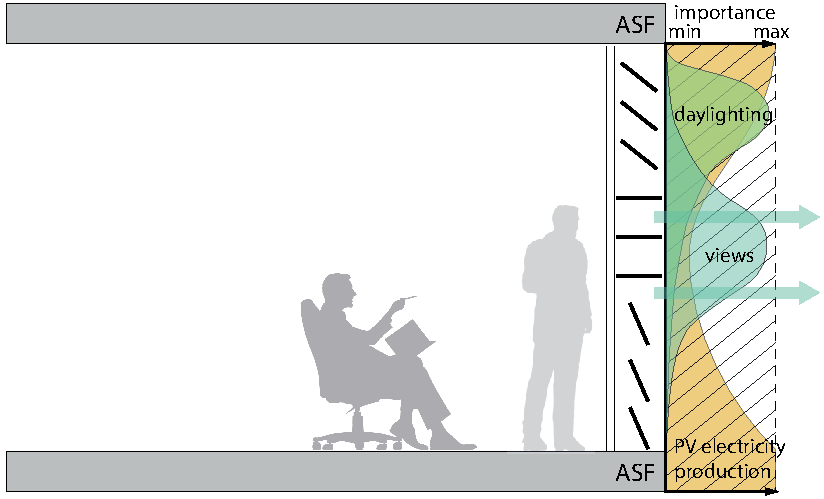
\includegraphics[width=8cm, trim= 0cm 0cm 0cm 0cm,clip]{facadeFunctions.pdf}
% \caption{The facade acting as a mediator between the interior and exterior environment, while fullfilling various functions \cite{nagy2015frontiers}}
% \label{fig:ASFschematic}
% \end{center}
% \end{figure}

% \begin{figure}
% \begin{center}
% \includegraphics[width=8cm, trim= 0cm 0cm 0cm 0cm,clip]{honr.jpg}
% \caption{An example of an ASF constructed at the House of Natural Resources \cite{nagy2015frontiers}}
% \label{fig:HoNR}
% \end{center}
% \end{figure}






\section{Methodology}
\label{ch:method}
% !TEX root = 99_main.tex

To study the electricity generation and building energy consumption, a 3D geometry of the room and solar facade is built using the Rhinoceros software \cite{Rhino}, and its parametric modelling plugin Grasshopper \cite{grasshopper}. The solar facade consists of 400mm CIGS square panels that can rotate in two degrees of freedom. On the horizontal axis the panels can move from 0$^{\circ}$ (closed) to 90$^{\circ}$ (open) position in steps of 22.5$^{\circ}$. In the vertical axis it can move from 45$^{\circ}$ to -45$^{\circ}$ in 22.5$^{\circ}$ steps. Existing ASF systems \cite{nagy2015frontiers} have independently actuated panels and a continuous range of actuation, however for simplicity we group all panels into one cluster that moves in unison. This leaves us with 25 possible dynamic configurations of the facade system. 

The building energy simulation is conducted using EnergyPlus \cite{energyplus} through the DIVA \cite{DIVA} interface. The geometric solar facade is interpreted in EnergyPlus as an external shading system. A solar radiance simulation is run in parallel with Ladybug \cite{roudsari2014ladybug}  which uses Radiance \cite{ward1994radiance} to determine the incident insolation on the solar facade. The approach enables us to calculate solar irradiance on the modules with high spatial resolution including the effect of module mutual shading as seen in Figure \ref{fig:radiation}. The results are coupled to an electrical circuit simulation of thin-film PV modules with sub-cell level representation \cite{hofer2015PVSEC}.

A simulation of each possible dynamic configuration of the facade is run for each hourly timestep of the year using using a weather file for Geneva, Switzerland \cite{genevaweatherfile}. The results are then post processed in Python \cite{python} to extract the configurations that minimise building energy consumption and maximise PV electricity production. A corresponding workflow can be seen in Figure \ref{fig:workflow}. 

%Johanes Comment for cyan text- This describes how it has been previously done. Please check the Ladybug/Radiance method used now and quickly describe it (calculation cumulative sky matrix for diffuse and beam radiation, etc). 


%  A cumulative sky matrix consisting of diffuse and direct radiation is calculated from the Geneva weather file \cite{genevaweatherfile} . This can be then used 
% \textcolor{cyan}{Reflected and diffuse light are taken into account using the global radiation data, visible sky fraction for each panel, and the reflection of surrounding elements - See Comments}.

% \begin{tikzpicture}[node distance = 3cm, auto]
% 	\node [decision] (rhino) {Rhino / Grasshopper};
% 	\node [block, left of=rhino] (geo) {Solar Facade Geometry};
% 	\node [block, below of=geo] (building) {Building Geometry};
% \end{tikzpicture}

% \begin{tikzpicture}[node distance = 2cm, auto]
%     % Place nodes
%     \node [block] (init) {initialize model};
%     \node [cloud, left of=init] (expert) {expert};
%     \node [cloud, right of=init] (system) {system};
%     \node [block, below of=init] (identify) {identify candidate models};
%     \node [block, below of=identify] (evaluate) {evaluate candidate models};
%     \node [block, left of=evaluate, node distance=3cm] (update) {update model};
%     \node [decision, below of=evaluate] (decide) {is best candidate better?};
%     \node [block, below of=decide, node distance=3cm] (stop) {stop};
%     % Draw edges
%     \path [line] (init) -- (identify);
%     \path [line] (identify) -- (evaluate);
%     \path [line] (evaluate) -- (decide);
%     \path [line] (decide) -| node [near start] {yes} (update);
%     \path [line] (update) |- (identify);
%     \path [line] (decide) -- node {no}(stop);
%     \path [line,dashed] (expert) -- (init);
%     \path [line,dashed] (system) -- (init);
%     \path [line,dashed] (system) |- (evaluate);
% \end{tikzpicture}

\begin{figure}
\begin{center}
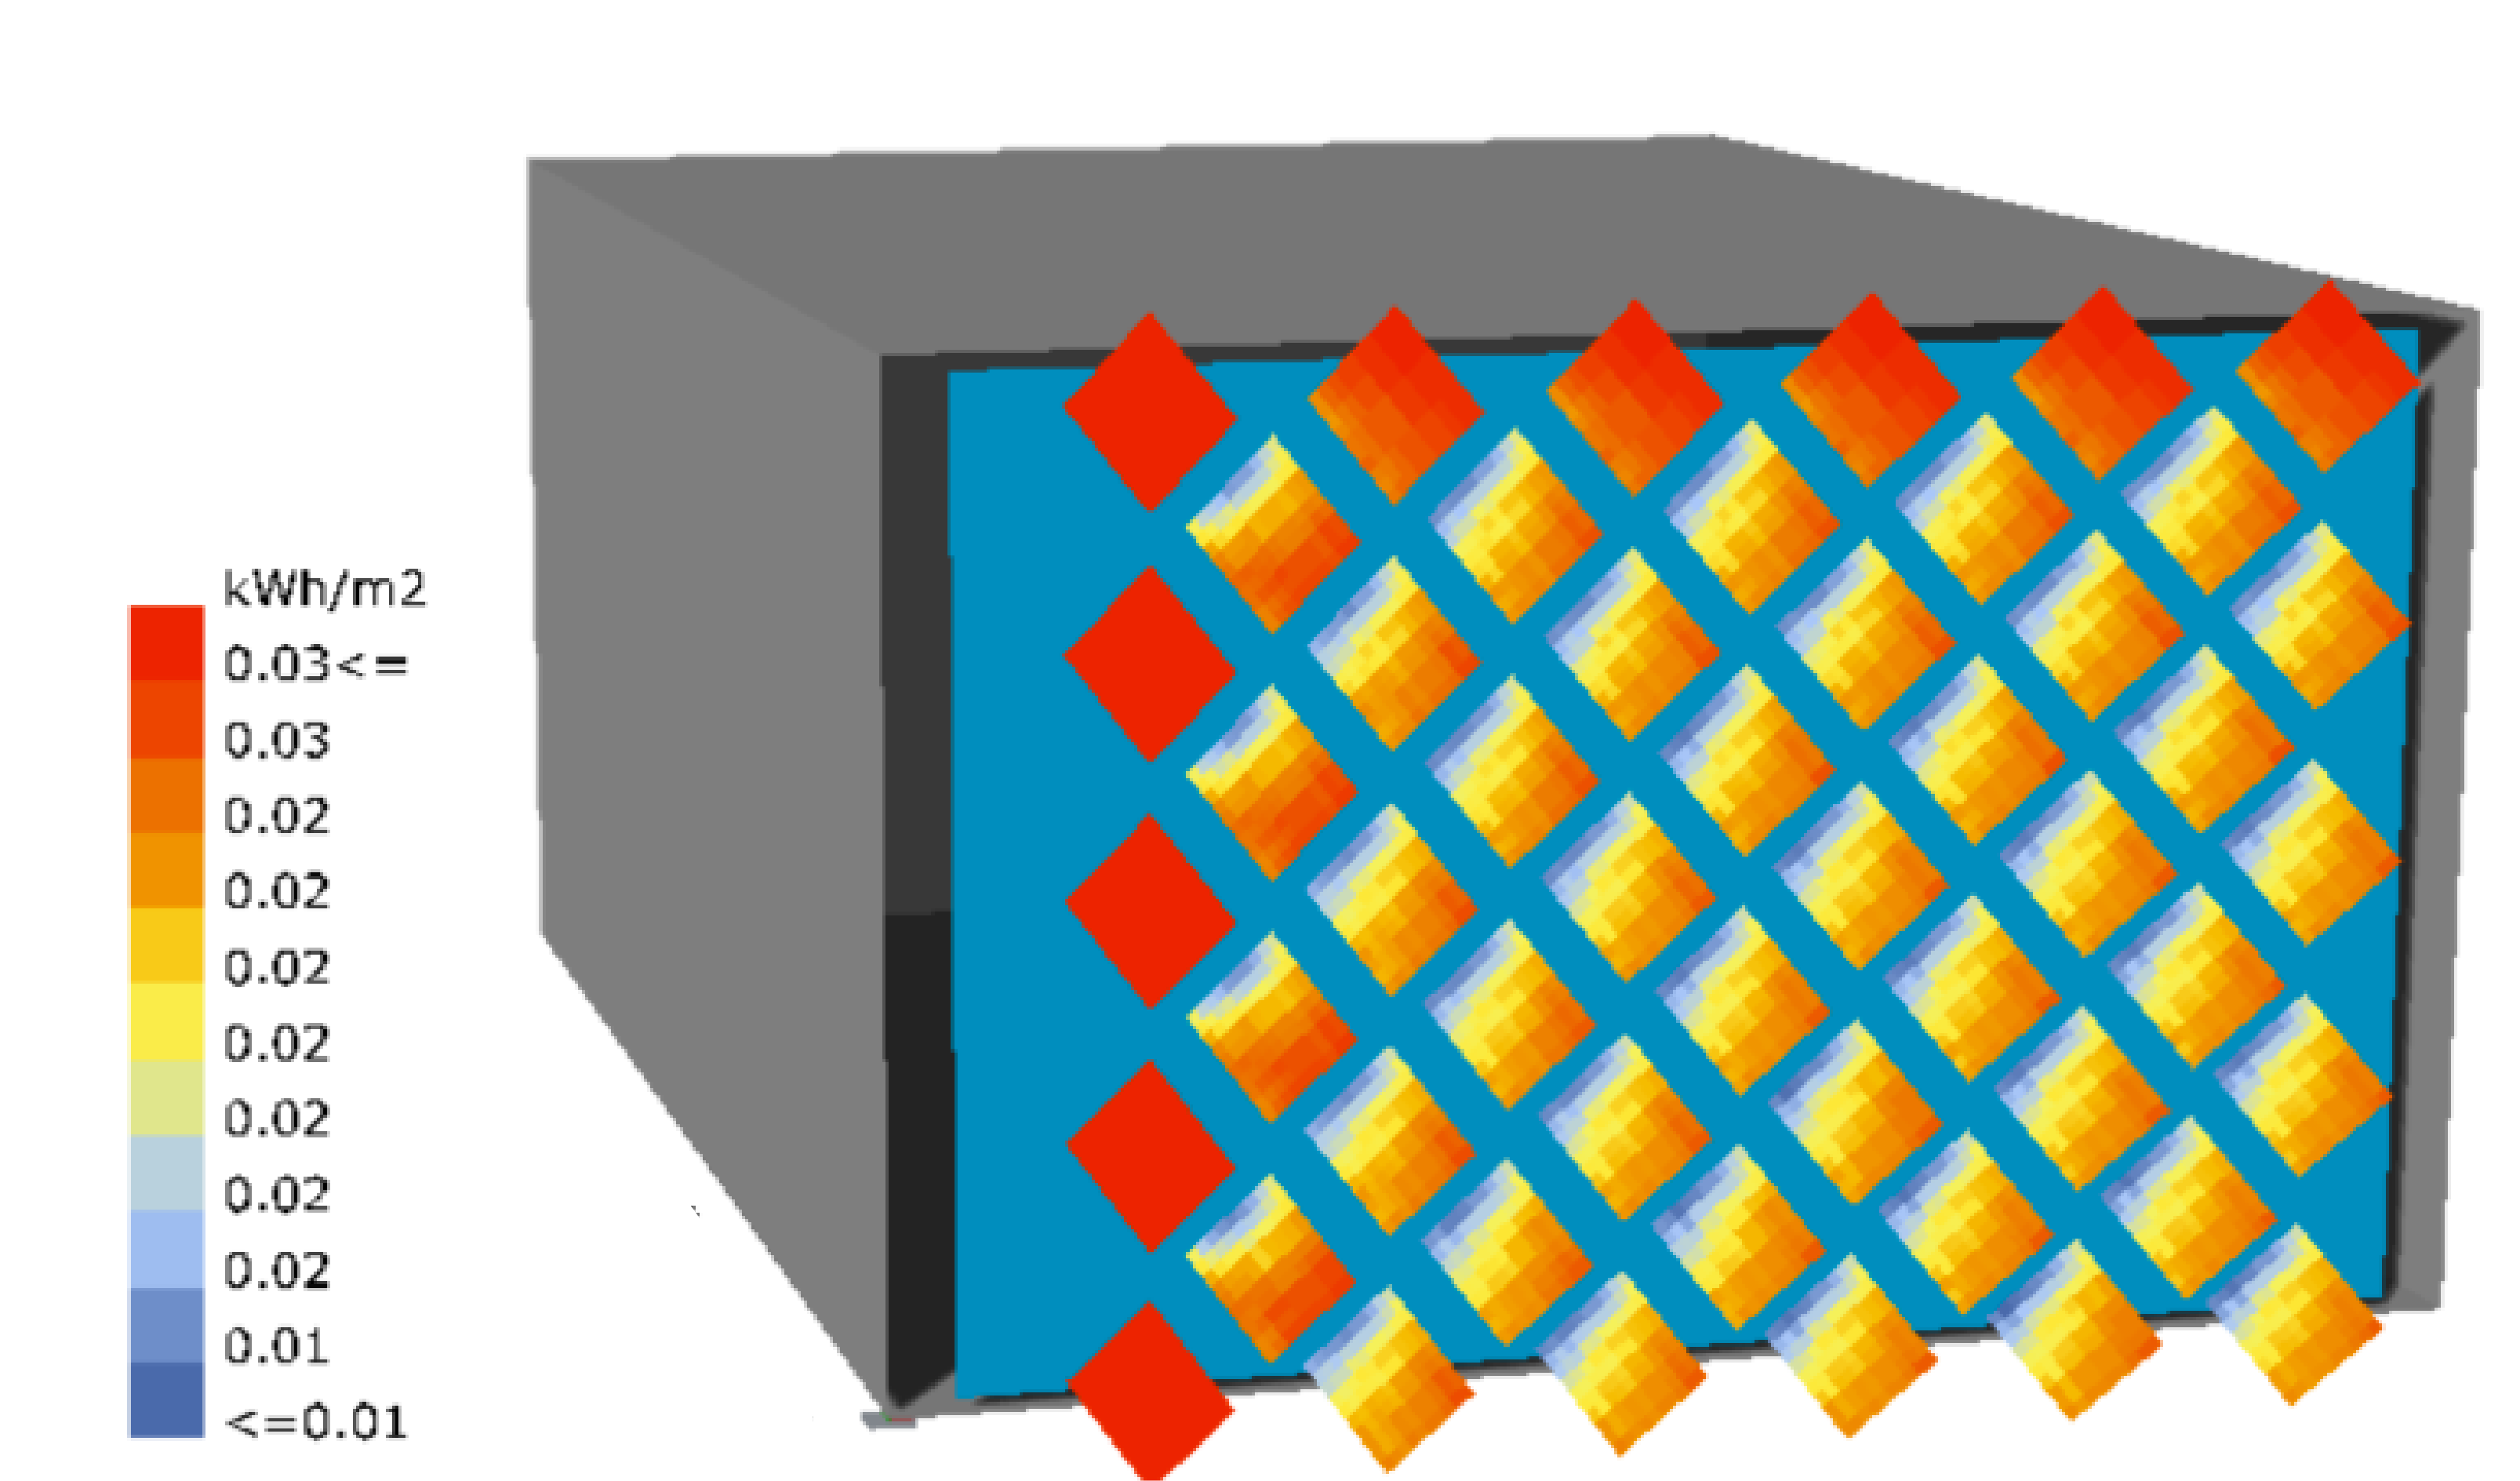
\includegraphics[width=10cm, trim= 0cm 0cm 0cm 0cm,clip]{radiationanalysis.png}
\caption{A simulation result showing module insolation from 14:00-15:00 on the 1st of January for the used weather file and a specific module orientation.}
\label{fig:radiation}
\end{center}
\end{figure}


\begin{figure}
\begin{center}
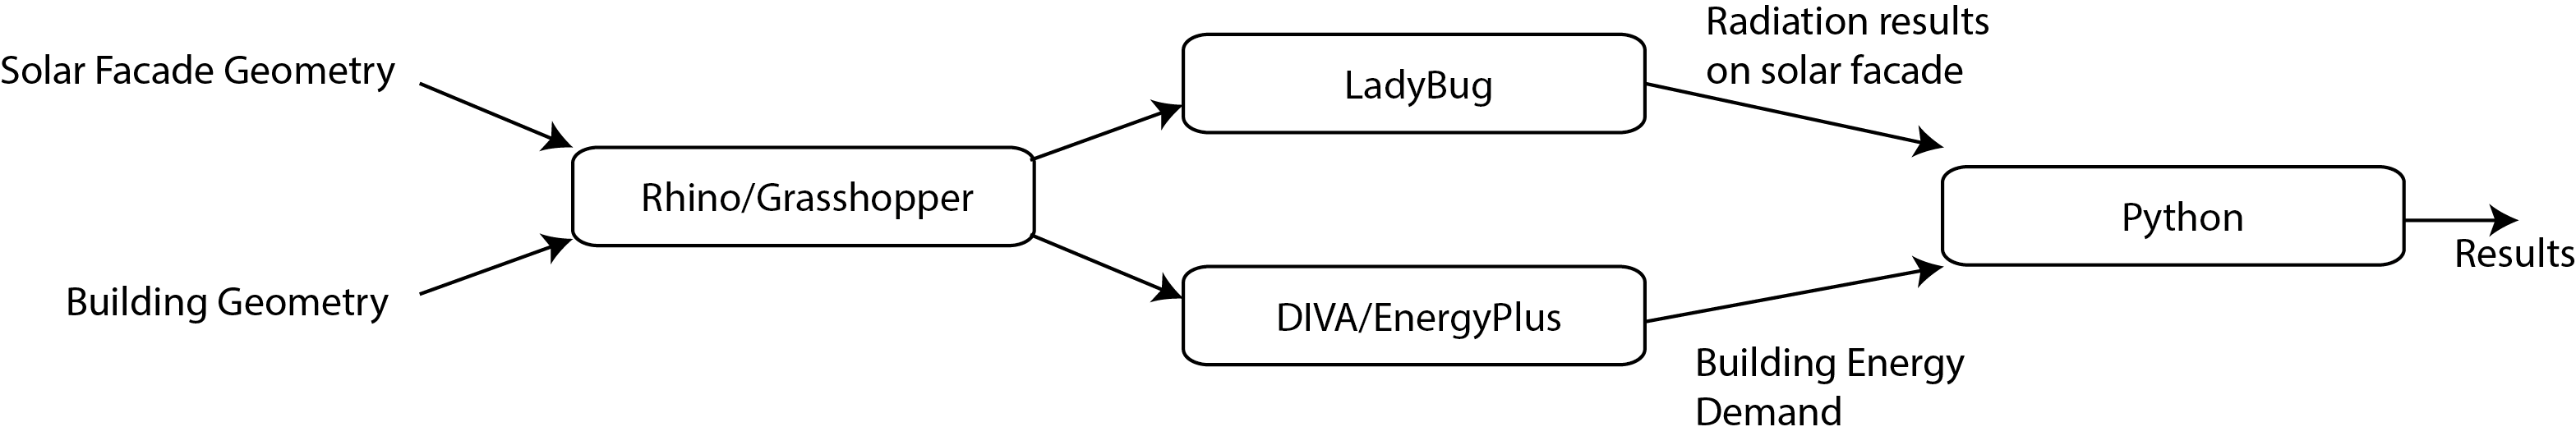
\includegraphics[width=15cm, trim= 0cm 0cm 0cm 0cm,clip]{workflow.png}
\caption{Simulation Workflow}
\label{fig:workflow}
\end{center}
\end{figure}

\section{Results}
\label{ch:results}
% !TEX root = 99_main.tex

% \begin{figure}
% \begin{center}
% 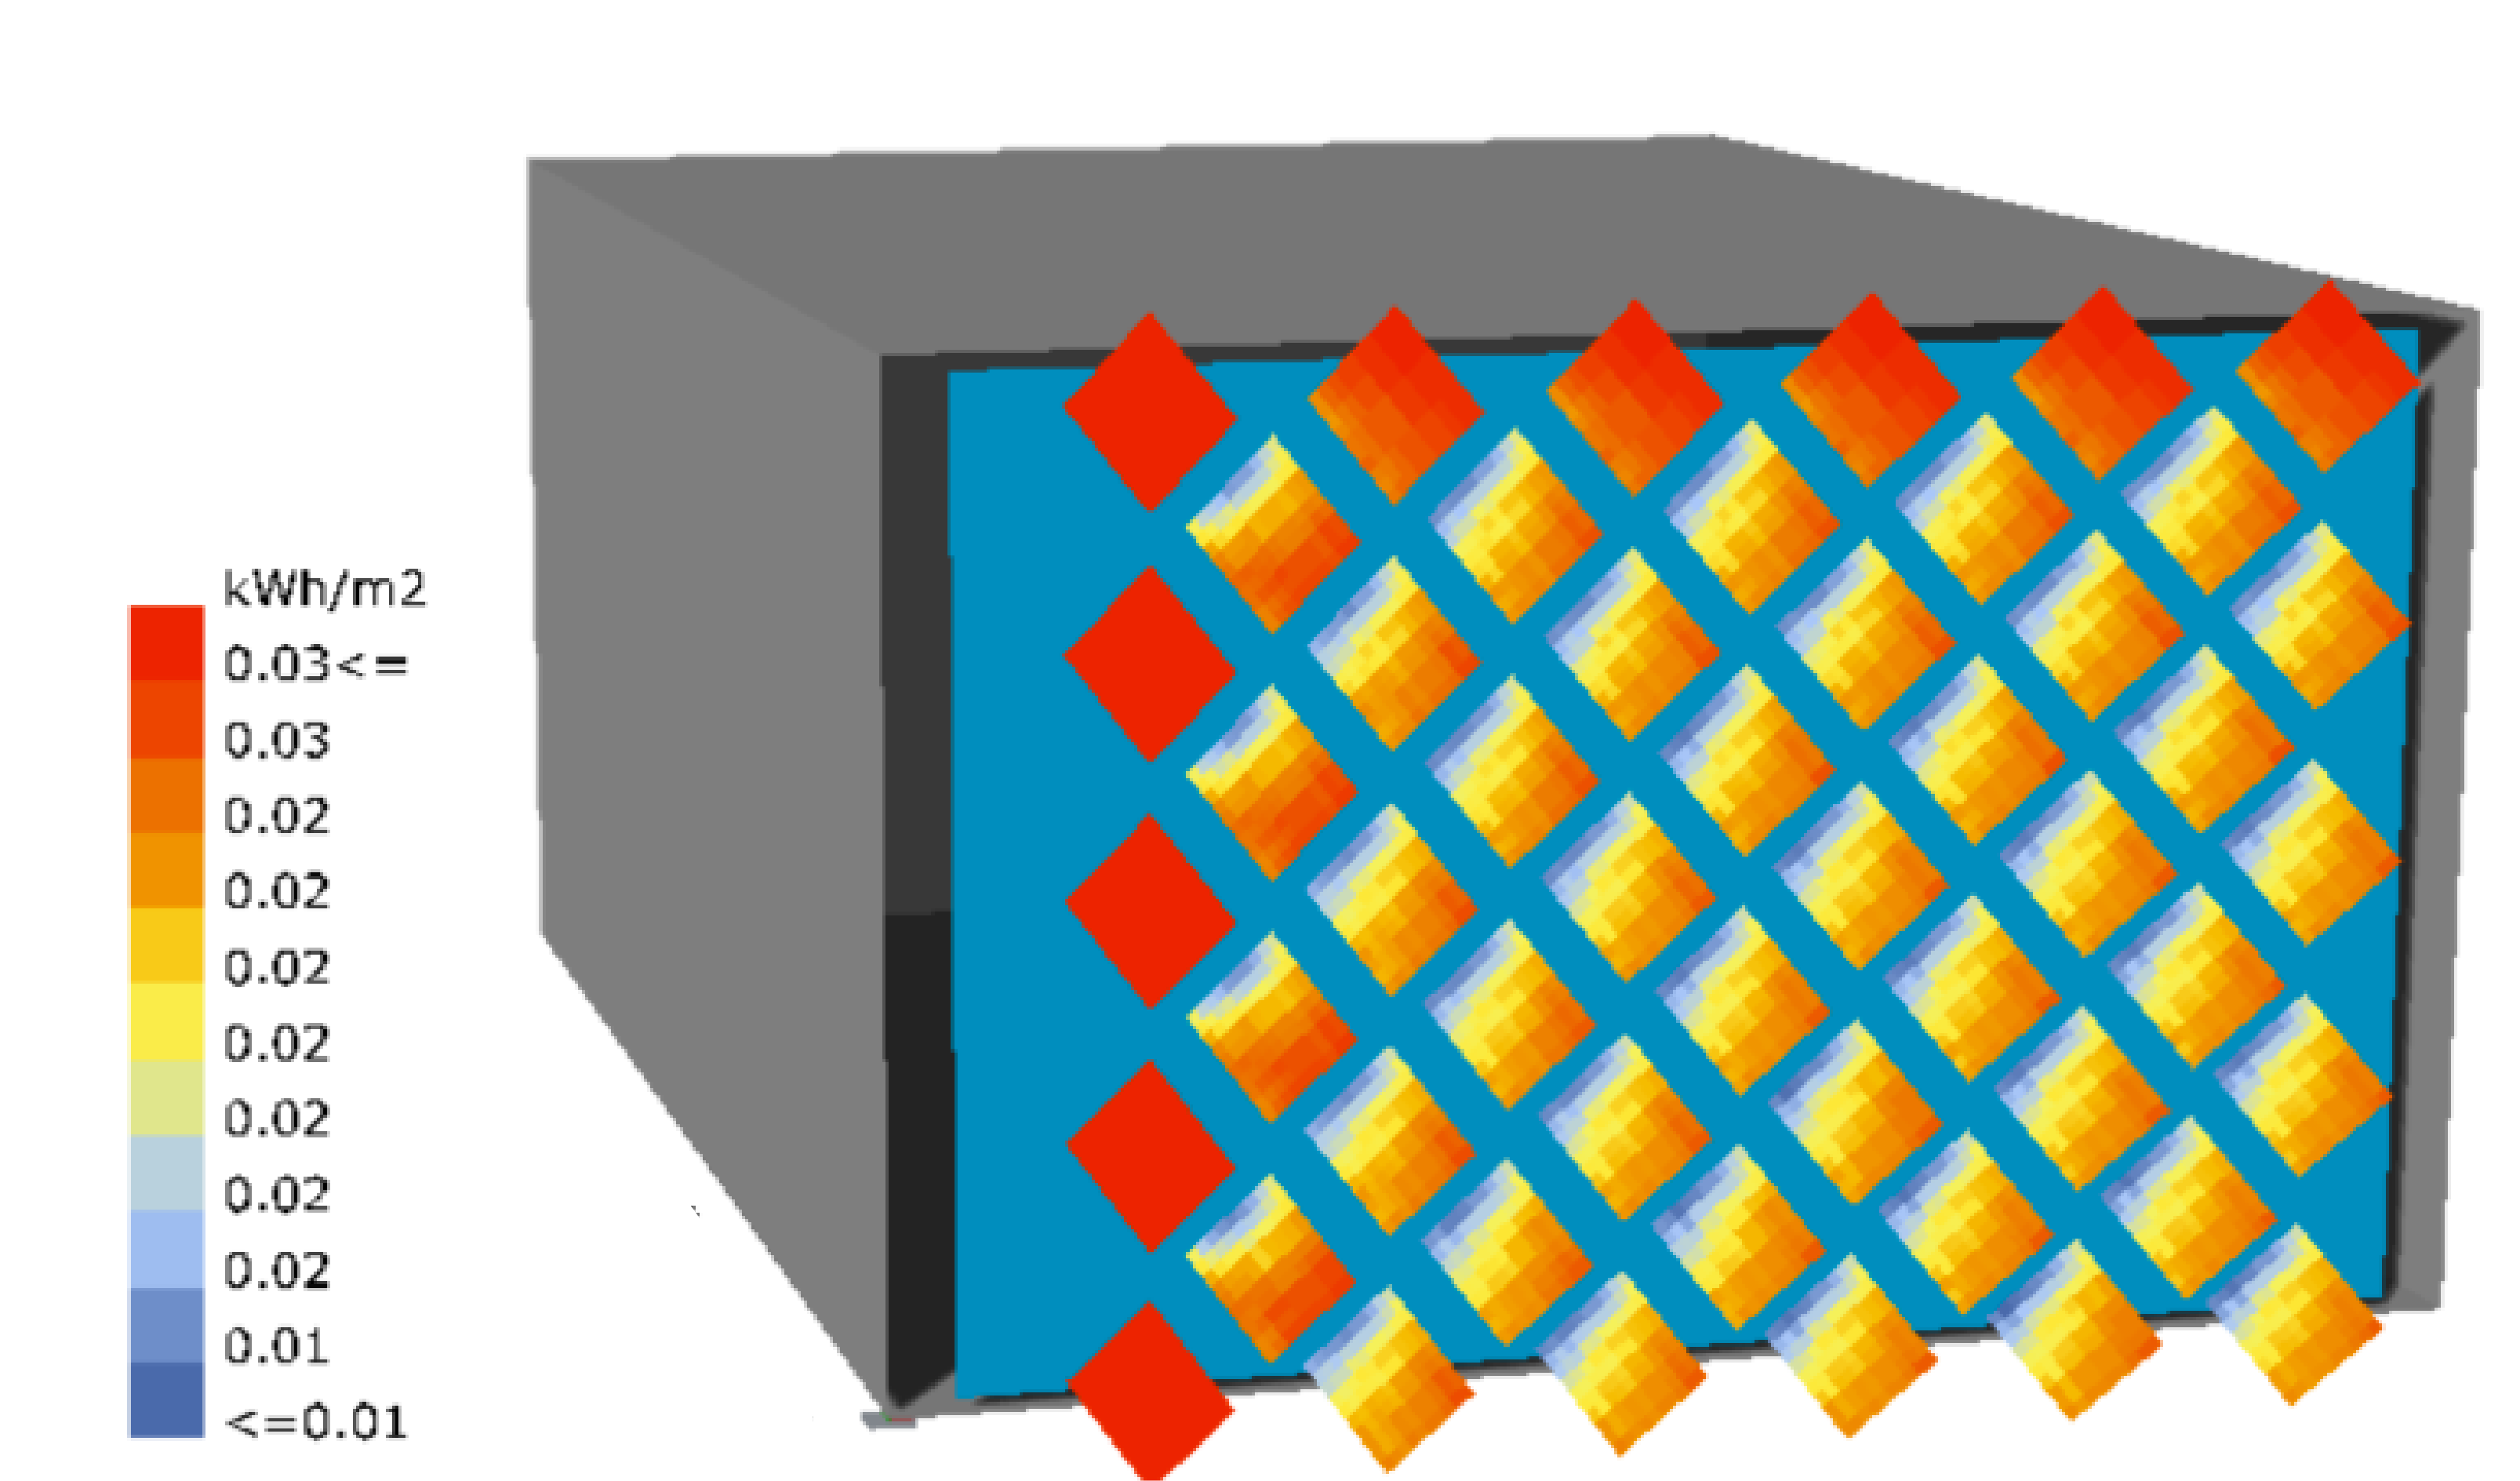
\includegraphics[width=8cm, trim= 0cm 0cm 0cm 0cm,clip]{radiationanalysis.png}
% \caption{Incident radiation on the PV panels. Light blue spots indicate areas of self shading}
% \label{fig:radiationanalysis}
% \end{center}
% \end{figure}


The optimal configurations of the ASF can be visualised using carpet-plots. Figure \ref{fig:carpetplot} details carpet-plots of the facade optimised to maximise PV generation, and minimise heating, cooling and lighting demands independently. We can see how open configurations (light coloured) are chosen to minimise the building heating demands during the winter months and early mornings of spring and autumn. Likewise closed configurations (dark colours) are the preferred solution to minimise the cooling demand during the summer months. Lighting control is only apparent during the twilight hours where the facade prefers an open position to avoid the use of artificial lighting. The PV optimisation [write as data comes in]...

\begin{figure}
\begin{center}
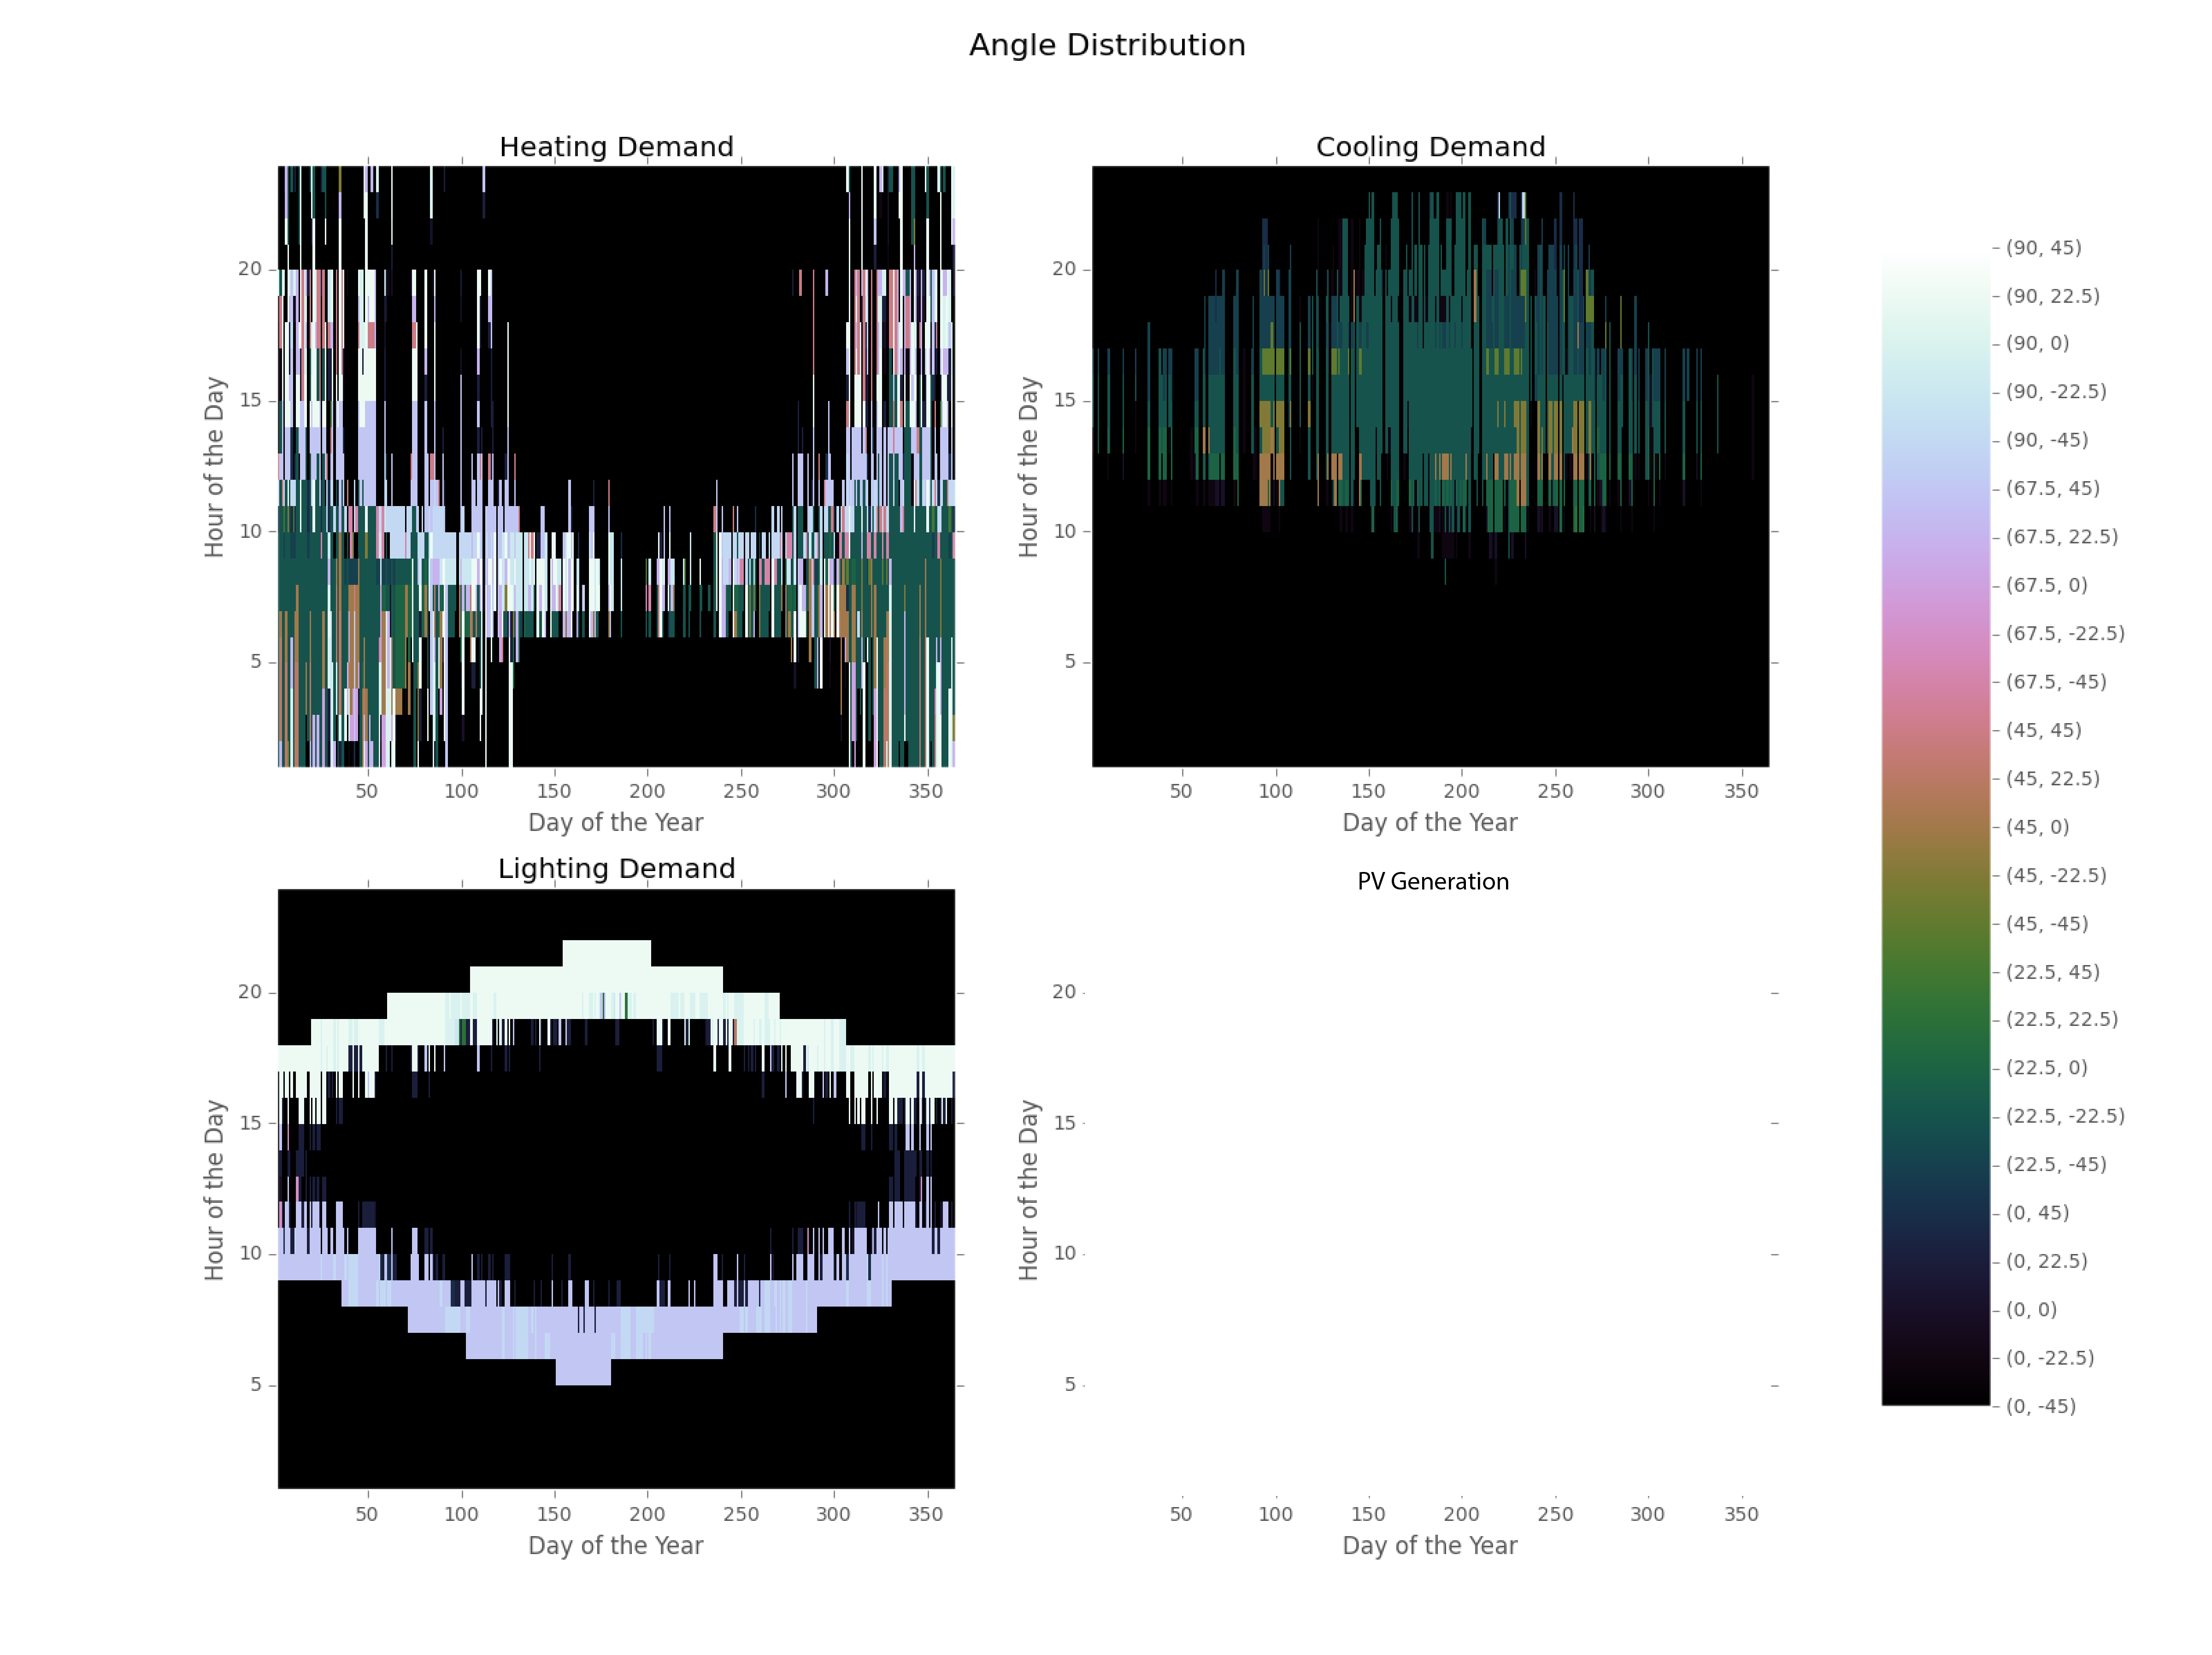
\includegraphics[width=15cm, trim= 0cm 0cm 0cm 0cm,clip]{carpetplot2.png}
\caption{A carpet plot detailing the optimal configuration to minimise the heating demand, cooling demand, lighting demand and maximise PV generation. Each configuration is represented by an angle of orientation around the x-axis and y-axis as seen in the legend.}
\label{fig:carpetplot}
\end{center}
\end{figure}

When the four optimisation cases are combined to achieve the configurations for total energy minimisation we get some interesting results. There is a conflict in the summer evenings between minimising lighting and cooling demands. Likewise, we also see a conflict between heating and PV production during the winter months....




% \section{Discussion}
% \label{ch:discussion}
% \input{5_discussion}

\section{Discussion and Conclusion}
\label{ch:conclusion}
% !TEX root = 99_main.tex

In this paper we present a simulation methodology to evaluate a dynamic photovoltaic shading system, combining both electricity generation, and the energy demand of the building. It is then coupled with a post processing python script to determine the optimum system configuration for control. The methodology can be applied to evaluate different PV system geometries, building systems, building typologies and climates.

The dynamic PV integrated shading system has clear advantages to a static system as it can adapt itself to the external environmental conditions. This enables it to orientate itself to the most energy efficient position. This, however, strongly depends on the general efficiency of the building. Decreasing the efficiency of the heating, cooling or lighting systems will give higher preference for configurations optimised for building thermal management through adaptive shading, than for PV electricity production.

%The use of LED lights, for example, reduces the weighting of the lighting energy demand. This would result in closed configurations optimised for cooling to over-ride the open positions. 

This work ultimately presents a methodology for the planning and optimisation of sophisticated adaptive BIPV systems. Future work will use this methodology to determine the environments and building typologies that could benefit from adaptive BIPV systems. 

%Moved to Introduction: The work presented in this paper is applied in the context of the Adaptive Solar Façade (ASF) project. The ASF is a lightweight PV shading system that can be easily installed on any surface of new or existing buildings. The ASF consists of a modular frame and pneumatically actuated panels to control glare and solar gain, as well as for two-axis PV tracking. It has been implemented at the ETH House of Natural Resources will be installed at the NEST HiLo building at EMPA (www.hilo.arch.ethz.ch). 

% \section{Outlook}
% \label{ch:outlook}

% [To be Decided]

% \section{Acknowledgments}
% \label{ch:acknowledgments}
% % !TEX root = 99_main.tex

%The authors would like to acknowledge the HiLo and HoNR project members for the design and construction of the ASF: Supermanoeuvre (Sydney Australia) and the Professorship of Architecture and Structures (BRG, ETH Zurich) for their work in designing the HiLo building; and the Institute of Structural Engineering (IBK, ETH Zurich) for their work in designing the HoNR building. We would also like to thank Stefanie Hellweg for her support in the LCA analysis. The authors would also like to thank other key contributors to the ASF Project: Bratislav Svetozarevic, Moritz Begle, Johannes Hofer, Nicola Offeddu, and Giovanni Bianchi. \\

%This research was partly funded by the Climate-KIC, Building Technologies Accelerator program.


% \section{Appendix}
% \label{ch:appendix}
% % !TEX root = 99_main.tex



%% appendix sections are then done as normal sections
%% \appendix
%% \section{}
%% \label{}

%% bibitems, please use
  \bibliographystyle{elsarticle-num} 
  \bibliography{references}

\end{document}
\endinput